\section{Experiments} \label{sec:exp}
% \wh{Experiments are too short. Can we expand this section with more details/insights?}
\vspace{-8pt}
For dynamic link property prediction, we include DyRep~\cite{trivedi2019dyrep},  TGN~\cite{rossi2020temporal}, CAWN~\cite{wanginductive}, TCL~\cite{wang2021tcl}, GraphMixer~\cite{congwe}, NAT~\cite{luoneighborhood}, TGAT~\cite{xu2020inductive} and two deterministic heuristics namely $\text{EdgeBank}_{\text{tw}}$ and $\text{EdgeBank}_{\infty}$~\cite{poursafaeitowards}. For dynamic node property prediction, we include DyRep,  TGN, and deterministic heuristics such as persistence forecast~\cite{salcedo2022persistence} and moving average~\cite{panch2018artificial}. Details about the above methods are presented in Appendix~\ref{app:methods}. The computing resources are discussed Appendix~\ref{sec:comp_resources}.
For the experimental results, we report the average and standard deviation across 5 different runs. \changed{We highlight the best results in bold and underline the second place results.}

% All results are averaged across 5 trials.
% and for reporting execution time, we use the timeit library in python. 


% Baseline for link prediction
% \begin{itemize}
%     \item Edgebank with frequency information (to make EdgeBank adoptable with ranking metrics)
%     \item Combine EdgeBank \& AdamicAdar: a better performance on new links?! (consider the characteristics of the neighboring nodes)
% \end{itemize}


\subsection{Dynamic Link Property Prediction} \label{sub:node_exp}


\begin{table*}[t]
\caption{\changed{Results for \emph{dynamic link property prediction} on \textcolor[HTML]{e7298a}{small} datasets.}}
\begin{subtable}[t]{0.5\textwidth}
\resizebox{\textwidth}{!}{
\begin{tabu}{ l | l l}
  \toprule
  \multirow{2}{*}{Method}    &   \multicolumn{2}{c}{\textbf{\textbf{MRR}}} \\
                           & Validation     & Test  \\
   \midrule
   \rowfont{\color{revised}}
    DyRep~\cite{trivedi2019dyrep}              & 0.072\scriptsize{$\pm$0.009}   & 0.050\scriptsize{$\pm$0.017} \\
    \rowfont{\color{revised}}
    TGN~\cite{rossi2020temporal}               & 0.435\scriptsize{$\pm$0.069}  & 0.396\scriptsize{$\pm$0.060}  \\
    \rowfont{\color{revised}}
    CAWN~\cite{wanginductive}                  & \underline{0.743}\scriptsize{$\pm$0.004}   & \underline{0.711}\scriptsize{$\pm$ 0.006} \\
    \rowfont{\color{revised}}
    TCL~\cite{wang2021tcl}                      & 0.198\scriptsize{$\pm$0.016}   & 0.207\scriptsize{$\pm$0.025}  \\
    \rowfont{\color{revised}}
    GraphMixer~\cite{congwe}                     & 0.113\scriptsize{$\pm$0.003}   & 0.118\scriptsize{$\pm$0.002}  \\
    \rowfont{\color{revised}}
    TGAT~\cite{xu2020inductive}                 &   0.131\scriptsize{$\pm$0.008} & 0.141\scriptsize{$\pm$0.007}\\
    \rowfont{\color{revised}}
    NAT~\cite{luoneighborhood}                   &  \textbf{0.773}\scriptsize{$\pm$0.011} &  \textbf{0.749}\scriptsize{$\pm$0.010}    \\
    
    % \midrule
    \rowfont{\color{revised}}
    $\text{EdgeBank}_{\text{tw}}$~\cite{poursafaeitowards}   & 0.600  & 0.571 \\
    \rowfont{\color{revised}}
    $\text{EdgeBank}_{\infty}$~\cite{poursafaeitowards}      & 0.527 & 0.495  \\
    \bottomrule
\end{tabu}
}
\caption{\textcolor[HTML]{e7298a}{\wikipedia} dataset with \emph{surprise index}: $0.108$ \\ (with \emph{all} negative edges per each positive edge).}
\label{tab:wiki}
\end{subtable}%
\begin{subtable}[t]{0.5\textwidth}
\resizebox{\textwidth}{!}{
\begin{tabu}{ l | l l}
  \toprule
  \multirow{2}{*}{Method}    &   \multicolumn{2}{c}{\textbf{\textbf{MRR}}} \\
                            & Validation     & Test  \\
   \midrule
   \rowfont{\color{revised}}
    DyRep~\cite{trivedi2019dyrep}             & 0.216\scriptsize{$\pm$0.031}  & 0.220\scriptsize{$\pm$0.030}  \\
    \rowfont{\color{revised}}
    TGN~\cite{rossi2020temporal}                & 0.313\scriptsize{$\pm$0.012}  & 0.349\scriptsize{$\pm$0.020}\\
    \rowfont{\color{revised}}
    CAWN\cite{wanginductive}               & 0.200\scriptsize{$\pm$0.001}   & 0.193\scriptsize{$\pm$0.001} \\
    \rowfont{\color{revised}}
    TCL~\cite{wang2021tcl}                & 0.199\scriptsize{$\pm$0.007} & 0.193\scriptsize{$\pm$0.009} \\
    \rowfont{\color{revised}}
    GraphMixer~\cite{congwe}         & \textbf{0.428}\scriptsize{$\pm$0.019}  & \textbf{0.521}\scriptsize{$\pm$0.015} \\
    \rowfont{\color{revised}}
    TGAT~\cite{xu2020inductive}     &  \underline{0.324}\scriptsize{$\pm$0.006} & \underline{0.355}\scriptsize{$\pm$0.012}  \\
    \rowfont{\color{revised}}
    NAT~\cite{luoneighborhood}      &  0.302\scriptsize{$\pm$0.011} &  0.341\scriptsize{$\pm$0.020}    \\
    % \midrule
    \rowfont{\color{revised}}
    $\text{EdgeBank}_{\text{tw}}$~\cite{poursafaeitowards}   & 0.0242 & 0.0253   \\
    \rowfont{\color{revised}}
    $\text{EdgeBank}_{\infty}$~\cite{poursafaeitowards}      & 0.0229 & 0.0229    \\
    \bottomrule
\end{tabu}
}
\caption{\textcolor[HTML]{e7298a}{\review} dataset with \emph{surprise index}: $0.987$ \\ (with \emph{100} negative edges per each positive edge).}
\label{tab:review}
\end{subtable}%
\vspace{-18pt}
\end{table*}




%results discussion for small scale link pred datasets
Table~\ref{tab:wiki} shows the performance of TG methods for dynamic link property prediction on the \wikipedia dataset. \wikipedia is an existing dataset where many methods achieve over-optimistic performance in the literature~\cite{rossi2020temporal,wanginductive,congwe}. 
\changed{With \name's evaluation protocol, there is now a clear distinction in model performance and NAT achieves the best result on this dataset. As \wikipedia is the smallest dataset in this task, it is computationally feasible to sample all possible destinations of a given source node. Thus, we compare the true destination with all possible negative destinations in this dataset. 
In Table~\ref{tab:review}, we report the results on \review where we sample 100 negative edges per positive edge. Here, we observe that many of the best performing methods on \wikipedia has a significant drop in performance including NAT, CAWN and Edgebank. More notably, the method rankings also changed significantly with GraphMixer and TGAT being the top two methods. This observation emphasizes the importance of dataset diversity when benchmarking TG methods. In Appendix~\ref{app:ns}, we conduct an ablation study on the effect of number of negative samples on the performance of dynamic link property prediction.}

\changed{One explanation for the significant performance reduction of some methods 
on \review is that it has a higher \emph{surprise index} compared to \wikipedia~(see Table~\ref{tab:stats-summarized}). The surprise index reflects the ratio of edges in the test set that have not been seen during training. Therefore, a dataset with a high surprise index requires more inductive reasoning, as most of the test edges are unobserved during training. As a heuristic that memorizes past edges, $\text{EdgeBank}$ performance is inversely correlated with the surprise index and it achieves higher performance when the suprise index of the dataset is low. 
% Lastly, another 
An interesting future direction is the investigation of the performance of certain category of methods with the surprise index. For example, the top two methods NAT and CAWN on wikipedia both utilizes features from the joint neighborhood of nodes in the queried edge~\cite{luoneighborhood}. On the \review dataset, the best performing TGAT is designed for inductive representation learning on temporal graph~\cite{xu2020inductive} which fits the inductive nature of \review which has high surprise index. 
}
% Most notably, the method rankings also changed significantly, with CAWN ranking amongst the lowest performing models on \review. These observations emphasize the importance of benchmarking methods on a variety of datasets offered by \name. One explanation for the general lower performance on \review is its higher \emph{surprise index} compared to that of \wikipedia (reported in Table~\ref{tab:stats-summarized}). The surprise index reflects the ratio of edges in the test set that have not been seen during training. Therefore, a dataset with a high surprise index requires more inductive reasoning, as most of the test edges are unseen. 
% As a heuristic that memorizes past edges, $\text{EdgeBank}$ performance is inversely correlated with the \emph{surprise index} and it achieves higher performance when the suprise index of the dataset is low. 


\begin{figure}[t]
\centering
\begin{subfigure}{.45\textwidth}
  \centering
  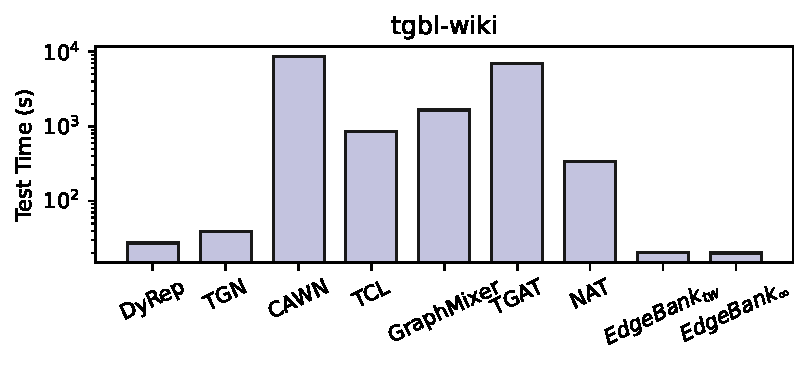
\includegraphics[width=\linewidth]{figs/time/tgbl-wiki_test_time.pdf}
  \caption{\textcolor[HTML]{e7298a}{\wikipedia} dataset.}
  \label{Fig:wiki_test}
\end{subfigure}%
\begin{subfigure}{.45\textwidth}
  \centering
  %
\includegraphics[width=.4\linewidth]{image1}
  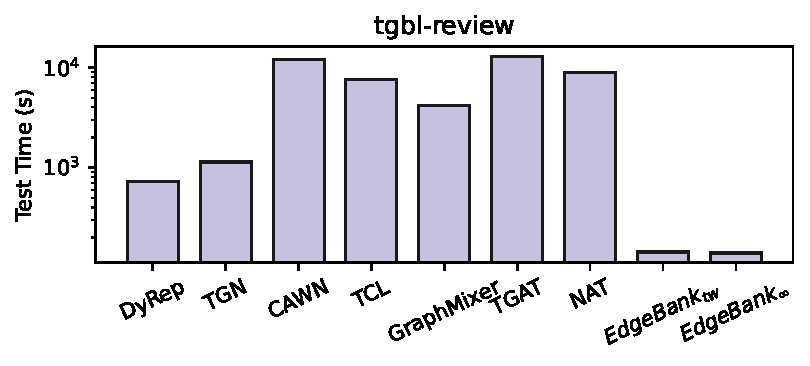
\includegraphics[width=\linewidth]{figs/time/tgbl-review_test_time.pdf}
  \caption{\textcolor[HTML]{e7298a}{\review} dataset.} 
  \label{Fig:review_test}
\end{subfigure}
\caption{ \changed{Test set inference time of TG methods can have up to two orders of magnitude difference.}}
\vspace{-8pt}
\end{figure}


\begin{figure}[t]
\centering
\begin{subfigure}{.45\textwidth}
  \centering
  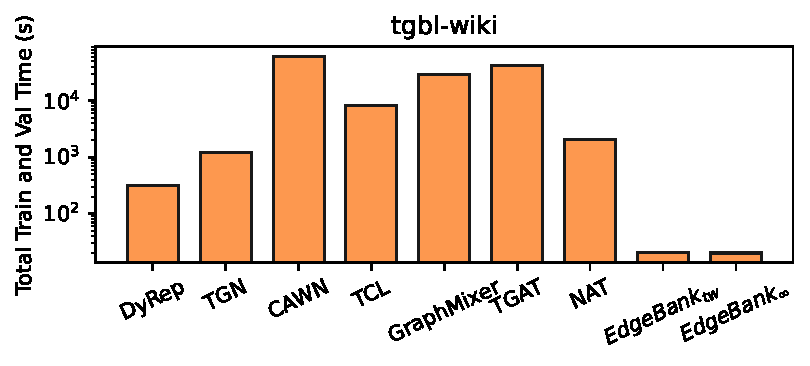
\includegraphics[width=\linewidth]{figs/time/tgbl-wiki_train_time.pdf}
  \caption{\textcolor[HTML]{e7298a}{\wikipedia} dataset.}
  \label{Fig:wiki_train}
\end{subfigure}%
\begin{subfigure}{.45\textwidth}
  \centering
  %
\includegraphics[width=.4\linewidth]{image1}
  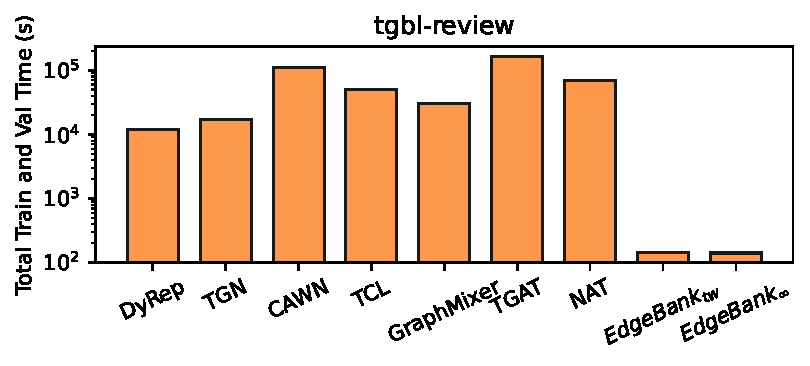
\includegraphics[width=\linewidth]{figs/time/tgbl-review_train_time.pdf}
  \caption{\textcolor[HTML]{e7298a}{\review} dataset.} 
  \label{Fig:review_train}
\end{subfigure}
\caption{\changed{Total train and validation time of TG methods can have two orders of magnitude difference.}}
\vspace{-10pt}
\end{figure}



Figure~\ref{Fig:wiki_test} and~\ref{Fig:review_test} show the inference time of different methods for the test set of \wikipedia and \review, respectively. \changed{Similarly, \changed{Figure~\ref{Fig:wiki_train} and~\ref{Fig:review_train}} show the total training and validation time of TG methods for \wikipedia and \review.  
Notice that as a heuristic baseline, $\text{EdgeBank}$ inference, train, or validation time is generally at least one order of magnitude lower than neural network based methods. 
We also observe an order of difference in inference time within TG methods.} 
We believe one important future direction is to improve the computational time of these models to be closer to baselines such as $\text{EdgeBank}$, which can better scale to large real-world temporal graphs.




%talk about performance degradation from validation set to test set
%CAWN drops significantly, also correlates with edgebank from previous work


%with v2 flight and coin results
\begin{table*}[t]
\caption{Results for \emph{dynamic link property prediction} task on \textcolor{blue}{medium} and \textcolor[HTML]{1b9e77}{large} datasets.} 
\label{tab:linkpred}
\centering
\resizebox{\textwidth}{!}{
  \begin{tabular}{l | l l | l l | l l }
  \toprule
  \multirow{3}{*}{Method} &  \multicolumn{2}{c|}{\textcolor{blue}{\coin}}  & \multicolumn{2}{c|}{\textcolor[HTML]{1b9e77}{\reddit}} & \multicolumn{2}{c}{\textcolor[HTML]{1b9e77}{\sky}} \\
  & \multicolumn{2}{c|}{\textbf{MRR}} & \multicolumn{2}{c|}{\textbf{MRR}} & \multicolumn{2}{c}{\textbf{MRR}}\\
                     & Validation  & Test                 & Validation   & Test            & Validation     & Test\\
  \midrule
    DyRep~\cite{trivedi2019dyrep}    & \underline{0.512}\scriptsize{$\pm$0.014}      & 0.452\scriptsize{$\pm$0.046}  
    & \underline{0.291}\scriptsize{$\pm$0.028}  & \underline{0.289}\scriptsize{$\pm$0.033}  &
    \underline{0.573}\scriptsize{$\pm$0.013}  & \underline{0.556}\scriptsize{$\pm$0.014}  \\
    
    TGN~\cite{rossi2020temporal}     & \textbf{0.607}\scriptsize{$\pm$0.014}   & \textbf{0.586}\scriptsize{$\pm$0.037} 
    & \textbf{0.356}\scriptsize{$\pm$0.019} & \textbf{0.379}\scriptsize{$\pm$0.021} & \textbf{0.731}\scriptsize{$\pm$0.010} & \textbf{0.705}\scriptsize{$\pm$0.020}     \\
    % \midrule
    $\text{EdgeBank}_{\text{tw}}$~\cite{poursafaeitowards} & 0.492  & \underline{0.580}  & 0.124  & 0.149  & 0.363  & 0.387 \\
    $\text{EdgeBank}_{\infty}$~\cite{poursafaeitowards}    & 0.315  & 0.359  & 0.109  & 0.129  & 0.166   & 0.167    \\

  \bottomrule
  \end{tabular}
}
\vspace{-8pt}
\end{table*}




% %with v1 flight and coin results
% \begin{table*}[t]
% \caption{Results for \emph{dynamic link property prediction} task on \textcolor{blue}{medium} and \textcolor[HTML]{1b9e77}{large} datasets.} 
% \label{tab:linkpred}
% \centering
% \resizebox{\textwidth}{!}{
%   \begin{tabular}{l | l l | l l | l l }
%   \toprule
%   \multirow{3}{*}{Method} &  \multicolumn{2}{c|}{\textcolor{blue}{\coin}}  & \multicolumn{2}{c|}{\textcolor[HTML]{1b9e77}{\reddit}} & \multicolumn{2}{c}{\textcolor[HTML]{1b9e77}{\sky}} \\
%   & \multicolumn{2}{c|}{\textbf{MRR}} & \multicolumn{2}{c|}{\textbf{MRR}} & \multicolumn{2}{c}{\textbf{MRR}}\\
%                      & Validation  & Test                 & Validation   & Test            & Validation     & Test\\
%   \midrule
%     DyRep~\cite{trivedi2019dyrep}    & \underline{0.507}\scriptsize{$\pm$0.029}      & 0.434\scriptsize{$\pm$0.038}  & \underline{0.291}\scriptsize{$\pm$0.028}  & \underline{0.289}\scriptsize{$\pm$0.033}  & \underline{0.528}\scriptsize{$\pm$0.022}  & \underline{0.543}\scriptsize{$\pm$0.024}  \\
    
%     TGN~\cite{rossi2020temporal}     & \textbf{0.594}\scriptsize{$\pm$0.023}   & \textbf{0.583}\scriptsize{$\pm$0.050} & \textbf{0.356}\scriptsize{$\pm$0.019} & \textbf{0.379}\scriptsize{$\pm$0.021} & \textbf{0.739}\scriptsize{$\pm$0.012} & \textbf{0.706}\scriptsize{$\pm$0.016}     \\
%     % \midrule
%     $\text{EdgeBank}_{\text{tw}}$~\cite{poursafaeitowards} & 0.492  & \underline{0.580}  & 0.124  & 0.149  & 0.388       & 0.364    \\
%     $\text{EdgeBank}_{\infty}$~\cite{poursafaeitowards}    & 0.315  & 0.359  & 0.109  & 0.129  & 0.166   & 0.167    \\

%   \bottomrule
%   \end{tabular}
% }
% \vspace{-8pt}
% \end{table*}




Table~\ref{tab:linkpred} shows the performance of TG methods on medium and large \name datasets. Note that some methods, including CAWN, TCL, and GraphMixer, ran out of memory on GPU for these datasets, thus their performance is not reported. Overall, TGN has the best performance on all of these three datasets. Surprisingly, the $\text{EdgeBank}$ heuristic is highly competitive on the \coin dataset where it even significantly outperforms DyRep. Therefore, it is important to include $\text{EdgeBank}$ as a baseline for all datasets. 
Another observation is that for medium and large \name datasets, there can be a significant performance change for a single model between the validation and test set. This is because \name datasets span over a long time~(such as \reddit, lasting 5 years) and one can expect that models need to deal with potential distribution shifts between the validation set and the test set. 

% Table~\ref{tab:linkpred} shows the performance of various methods on \name dynamic link prediction task. \wikipedia dataset is a common dataset used in the current evaluation. With the improved evaluation from \name, we see that methods now have clear performance difference as opposed to all having high performance. \wh{Do you have ROC-AUC numbers to make this argument stronger?} We observe that the heuristics baseline EdgeBank is a strong contender in datasets with low surprise index such as \wikipedia and \coin while having poor performance those with high surprise index such as \review and \reddit. \wh{Grammer might be wrong}
% Figure~\ref{Fig:wiki_test} shows a huge difference between the computational time required for inference amongst different TG methods with the most drastic being two orders of magnitude different. 

%results discussion for medium large datasets in link pred 

% \begin{figure*}[t]
%     \begin{center}
%         \centerline{
\includegraphics[width=0.5\textwidth]{figs/wiki_test.png
% }} %\vspace{-15pt}
%         \caption{Test computational time reported across all methods in \textcolor[HTML]{e7298a}{\wikipedia} dataset. \\
%         Inference time of models can be two orders of magnitude different. \wh{Put Fig 4 and 5 side-by-side to save space.} }
%         \label{Fig:wiki_test}
%     \end{center}
% \end{figure*}


% \begin{figure*}[t]
%     \begin{center}
%         \centerline{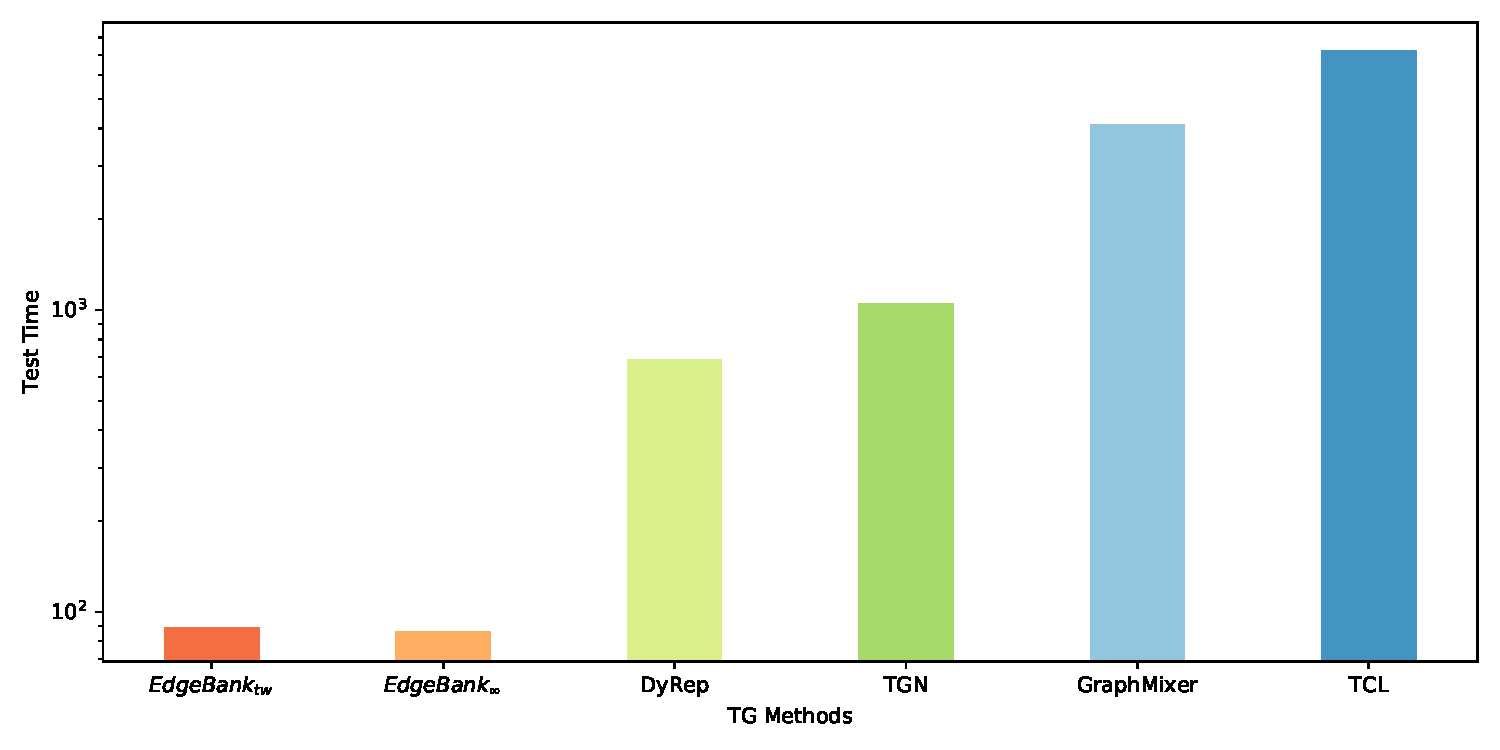
\includegraphics[width=0.5\textwidth]{figs/review_test.pdf}} %\vspace{-15pt}
%         \caption{Test computational time reported in \textcolor[HTML]{e7298a}{\review} dataset.}
%         \label{Fig:review_test}
%     \end{center}
% \end{figure*}





% \textcolor{green}{[FP: the relation of surprise and edgebank is somehow clear; however, there's also a relation between recurrence and the performance; for example, when edges repeat consistently (i.e., low surprise and high recurrence), edgebank performs well (comparing wikipedia and amazonreview). Surprise relates to the inability of edgebank to predict new edges, reocurrence relates to its inability of distinguishing non-existing edges.]}


% We observe that the simple baseline Edgebank is a strong contender on this dataset even having the best validation performance. Secondly, we observe that in both \wikipedia and \review datasets, there is a significant performance difference between validation and test set. In this likely due to the distribution shift in temporal graphs over time and models should be able to adapt to the change. 




\subsection{Dynamic Node Property Prediction}



\begin{table*}[t]
\caption{\changed{\emph{Node affinity prediction} results.}} 
\label{tab:nodepred}
\centering
\resizebox{\textwidth}{!}{
  \begin{tabu}{l | l l | l l | l l | l l}
  \toprule
  \multirow{3}{*}{Method} &  \multicolumn{2}{c|}{\textcolor[HTML]{e7298a}{\trade}}  & \multicolumn{2}{c|}{\textcolor{blue}{\fm}} & \multicolumn{2}{c|}{\textcolor[HTML]{1b9e77}{\subreddit}} & \multicolumn{2}{c}{\textcolor[HTML]{1b9e77}{\token}} \\
  \rowfont{\color{revised}}
   & \multicolumn{2}{c|}{\textbf{NDCG@10}}       & \multicolumn{2}{c|}{\textbf{NDCG@10}} & \multicolumn{2}{c}{\textbf{NDCG@10}} & \multicolumn{2}{c}{\textbf{NDCG@10}} \\
       & Validation  & Test                & Validation    & Test             & Validation      & Test & Validation      & Test \\
    \midrule
    \rowfont{\color{revised}}
    DyRep~\cite{trivedi2019dyrep}    & 0.394\scriptsize{$\pm$0.001} & 0.374\scriptsize{$\pm$0.001} & 0.357\scriptsize{$\pm$0.001} & 0.351\scriptsize{$\pm$0.001} & 0.344\scriptsize{$\pm$ 0.001} & 0.312\scriptsize{$\pm$ 0.001}
    & 0.151\scriptsize{$\pm$ 0.006} & 0.141\scriptsize{$\pm$ 0.006}\\

    \rowfont{\color{revised}}
    TGN~\cite{rossi2020temporal}      & 0.395\scriptsize{$\pm$0.002} & 0.374\scriptsize{$\pm$0.001} & \underline{0.403}\scriptsize{$\pm$0.010} & \underline{0.367}\scriptsize{$\pm$0.058} & \underline{0.379}\scriptsize{$\pm$ 0.004} & 0.315\scriptsize{$\pm$ 0.020}  
    & 0.189\scriptsize{$\pm$ 0.005} & 0.169\scriptsize{$\pm$ 0.006}\\
    % \midrule
    \rowfont{\color{revised}}
    persistence Fore.~\cite{salcedo2022persistence} & \textbf{0.860}  & \textbf{0.855} & 0.350    & 0.357 & \underline{0.380}   & \underline{0.369} & \underline{0.403} & \underline{0.430}\\
    \rowfont{\color{revised}}
    Moving Avg.~\cite{panch2018artificial}      & \underline{0.841}   & \underline{0.823} & \textbf{0.499} & \textbf{0.509} & \textbf{0.574}    & \textbf{0.559} & \textbf{0.491} & \textbf{0.508}\\
  \bottomrule
  \end{tabu}
}
\vspace{-8pt}
\end{table*}



% with 4 significant digits
% \begin{table*}[t]
% \caption{\emph{Dynamic node property prediction} results across 5 trials.} 
% \label{tab:nodepred}
% \centering
% \resizebox{\textwidth}{!}{
%   \begin{tabular}{l | l l | l l | l l }
%   \toprule
%   \multirow{3}{*}{Method} &  \multicolumn{2}{c|}{\textcolor[HTML]{e7298a}{\trade}}  & \multicolumn{2}{c|}{\textcolor{blue}{\fm}} & \multicolumn{2}{c}{\textcolor[HTML]{1b9e77}{\subreddit}} \\
%    & \multicolumn{2}{c|}{\textbf{NDCG@10} (\%)}       & \multicolumn{2}{c|}{\textbf{NDCG@10} (\%)} & \multicolumn{2}{c}{\textbf{NDCG@10} ($10^{-4}$)} \\
%        & Validation  & Test                & Validation    & Test             & Validation      & Test \\
%        \midrule
%     DyRep~\cite{trivedi2019dyrep}    & 0.1856\scriptsize{$\pm$0.0004} & 0.1688\scriptsize{$\pm$0.0004} & 0.1594\scriptsize{$\pm$0.0004} & 0.1810\scriptsize{$\pm$0.0006} & 0.5077\scriptsize{$\pm$ 0.0001} & 0.4635\scriptsize{$\pm$ 0.0002} \\
%     TGN~\cite{rossi2020temporal}      & 0.1851\scriptsize{$\pm$0.0018} & 0.1682\scriptsize{$\pm$0.0006} & \textbf{0.1763}\scriptsize{$\pm$0.0054} & \textbf{0.1957}\scriptsize{$\pm$0.0105} & 0.5587\scriptsize{$\pm$ 0.0054} & 0.4458\scriptsize{$\pm$ 0.0776}  \\
%     % \midrule
%     persistence Forecast & \textbf{0.4049}  & \textbf{0.3856} & 0.1070    & 0.1261 & 0.5606   & 0.5482 \\
%     Moving Average      & 0.3956   & 0.3711 & 0.1641 & 0.1930 & \textbf{0.8471}    & \textbf{0.8311} \\
%   \bottomrule
%   \end{tabular}
% }
% \end{table*}
% \wh{Better organize the position of the tables}
Table~\ref{tab:nodepred} shows the performance of various methods on the \changed{node affinity prediction task in the dynamic node property prediction category.}
% As node level tasks have received less attention compared to edge level tasks in the literature, extending edge embedding based methods such as CAWN and GraphMixer to the dynamic node property prediction task is non-trivial, thus they are not included in these experiments. 
\changed{As node level tasks have received less attention compared to edge level tasks in the literature, adopting methods that are specially designed for link prediction to this task is non-trivial. 
As a result, these methods are omitted in this section. 
Considering Table~\ref{tab:nodepred}, the key observation is that simple heuristics like persistence forecast and moving average are strong contenders to TG methods such as DyRep and TGN. 
Notably, persistence forecast is SOTA on \trade while moving average is the best performing on other datasets. TGN is second place on \fm dataset. Different from link prediction where the existence of a link is casted as binary classification, the node affinity prediction task compares the likelihood or weight that the model assigns to different target nodes (mostly positive links). These results highlight the need for the future development of TG methods that can acquire flexible node representations capable of learning how user preferences evolve over time.}

% One key observation is that despite being simple heuristics, both persistence forecast and moving average are strong contenders to TG methods such as DyRep and TGN. Notably, persistence forecast is SOTA on \trade while moving average is SOTA on \reddit. On the \fm dataset, TGN outperforms other methods, while moving average is a close second. This observation calls for the development of future TG methods for node-centric tasks such as node property prediction. 


% We observe that both persistence forecast and moving average remain strong baselines when compared to TGN. This is likely because current TG models are often developed for link prediction tasks. This calls for the development of future methods for node-centric tasks such as node property prediction. 


% %\textbf{It is persistence not Persitant}
% \begin{table*}[t]
% \caption{Dynamic Node Property Prediction Results reported from 5 trials.} 
% \label{tab:nodepred}
% \centering
% \resizebox{0.6\textwidth}{!}{
%   \begin{tabular}{l | l l l}
%   \toprule
%   \multirow{2}{*}{Dataset}  & \multirow{2}{*}{Method}                     &   \multicolumn{2}{c}{\textbf{NDCG@10} (\%)} \\
%    &                               & Validation    & Test \\
%   \midrule
%   \multirow{4}{*}{\trade} & TGN                 & 0.1851\scriptsize{$\pm$0.0018} & 0.1682\scriptsize{$\pm$0.0006} \\
%                           & DyRep               & 0.1856\scriptsize{$\pm$0.0004} & 0.1688\scriptsize{$\pm$0.0004} \\
%                           & persistence Forecast & \textbf{0.4049}\scriptsize{$\pm$0.0000}  & \textbf{0.3856}\scriptsize{$\pm$0.0000} \\
%                           & Moving Average & 0.3956\scriptsize{$\pm$0.0000}   & 0.3711\scriptsize{$\pm$0.0000}  \\
%   \midrule
%   % Dataset &                 Method              & Val NDCG @ 10 (\%)    & Test NDCG @ 10 (\%)\\
%   \multirow{4}{*}{\fm}    & TGN                 & \textbf{0.1763}\scriptsize{$\pm$0.0054} & \textbf{0.1957}\scriptsize{$\pm$0.0105} \\
%                           & DyRep               & 0.1594\scriptsize{$\pm$0.0004} & 0.1810\scriptsize{$\pm$0.0006}  \\
%                           & persistence Forecast & 0.1070\scriptsize{$\pm$0.0}    & 0.1261\scriptsize{$\pm$0.0} \\
%                           & Moving Average & 0.1641\scriptsize{$\pm$0.0}    & 0.1930\scriptsize{$\pm$0.0} \\
% \midrule
%     % Dataset &                 Method              & Val NDCG @ 10 ($e^{-4}$)   & Test NDCG @ 10 ($e^{-4}$)\\\
%       &                     &   \multicolumn{2}{c}{\textbf{NDCG@10 ($10^{-4}$)}} \\
%     \midrule
%     \multirow{4}{*}{\reddit}    & TGN           & 0.5587\scriptsize{$\pm$ 0.0054} & 0.4458\scriptsize{$\pm$ 0.0776} \\
%                           & DyRep               & 0.5077\scriptsize{$\pm$ 0.0001} & 0.4635\scriptsize{$\pm$ 0.0002}\\
%                           & persistence Forecast & 0.5606\scriptsize{$\pm$0.0}    & 0.5482\scriptsize{$\pm$0.0} \\
%                           & Moving Average & \textbf{0.8471}\scriptsize{$\pm$0.0}    & \textbf{0.8311}\scriptsize{$\pm$0.0} \\
    

%   \bottomrule
%   \end{tabular}
% }
% \end{table*}


% \begin{table*}[t]
% \caption{Node Property Prediction Results reported from 5 trials.} 
% \label{tab:nodepred}
%   \begin{tabular}{l | l l l l l}
%   \toprule
%   Dataset &                 Method              & Val NDCG      & Test NDCG       & Test Time (secs) & Training Time (secs) \\
%   \midrule
%   \multirow{3}{*}{\trade} & TGN                 & 0.00183       & 0.00168       & 2.4  & 13.8 \\
%                           & Persistant Forecast & 0.00394       & 0.00376       & 0.2   &  1.1\\
%                           & Moving Average (7)  & 0.00386       & 0.00365       & 0.2   & 1.4 \\
%   \midrule
%   \multirow{4}{*}{\fm}    & TGN                 & 0.00155       & 0.00171       & 77.5  & 381.1 \\
%                           & DyRep               & 0.00147       & 0.00166       & 78.5  & 327.7 \\
%                           & Persistant Forecast & 0.00107       & 0.00126       & 0.9   & 53.5 \\
%                           %& Moving Average (3)  & 0.00152       & 0.00179       & xxx   & xxx \\
%                           & Moving Average (7)  & 0.00167       & 0.00196       & 11.0   & 60.7 \\

%   \bottomrule
%   \end{tabular}
% \end{table*}




% \begin{table*}[t]
% \caption{Dynamic Link Prediction Results reported from 5 trials.} 
% \label{tab:linkpred}
% \centering
% \resizebox{0.6\textwidth}{!}{
%   \begin{tabular}{l | l l l }
%   \toprule
%   \multirow{2}{*}{Dataset}  & \multirow{2}{*}{Method}                     &   \multicolumn{2}{c}{\textbf{MRR}} \\
%    &                   & Validation     & Test  \\
%   \midrule
%   % \multirow{7}{*}{\wikipedia} & DyRep                           & 0.411\scriptsize{$\pm$0.015}   & 0.366\scriptsize{$\pm$0.014} \\
%   %                             & TGN                             & 0.737\scriptsize{$\pm$0.004}  & 0.721\scriptsize{$\pm$0.004}  \\
%   %                             & CAWN                            & \textbf{0.794}\scriptsize{$\pm$0.014}   & \textbf{0.791}\scriptsize{$\pm$ 0.015} \\
%   %                             & TGAT                            & 0.690\scriptsize{$\pm$0.011} &  0.668\scriptsize{$\pm$0.0114}\\
%   %                             & TCL                             & 0.734\scriptsize{$\pm$0.007}   & 0.712\scriptsize{$\pm$0.007}  \\
%   %                             & GraphMixer                      & 0.707\scriptsize{$\pm$0.014}   & 0.701\scriptsize{$\pm$0.014}  \\
%   %                             & $\text{EdgeBank}_{\text{tw}}$   & 0.641  & 0.641 \\
%   %                             & $\text{EdgeBank}_{\infty}$      & 0.551 & 0.538  \\
                              
%   %   \midrule
%   %   \multirow{5}{*}{\review}  & DyRep              & 0.356\scriptsize{$\pm$0.016}  & 0.367\scriptsize{$\pm$0.013}  \\
%   %                             & TGN                & \textbf{0.465}\scriptsize{$\pm$0.010}  & \textbf{0.532}\scriptsize{$\pm$0.020}\\
%   %                             % & CAWN               & xxx \scriptsize{xxx}   & xxx\scriptsize{xxx} \\
%   %                             & GraphMixer         & 0.411\scriptsize{$\pm$0.025}  & 0.514\scriptsize{$\pm$0.020} \\
%   %                             & TCL                & 0.194\scriptsize{$\pm$0.012} & 0.200 \scriptsize{$\pm$0.010} \\
%   %                             & $\text{EdgeBank}_{\text{tw}}$   & 0.0894 & 0.0836     \\
%   %                             & $\text{EdgeBank}_{\infty}$      & 0.0786      & 0.0795      \\

%   %   \midrule
%     \multirow{4}{*}{\coin}   & DyRep             & xxx       & xxx      \\
%                               & TGN              & 0.594\scriptsize{$\pm$0.023}   & 0.583\scriptsize{$\pm$0.050} \\
%                               & $\text{EdgeBank}_{\text{tw}}$  & 0.492     & 0.580   \\
%                               & $\text{EdgeBank}_{\infty}$     & 0.315     & 0.359      \\

%     \midrule
%     \multirow{4}{*}{\reddit}  & DyRep              & 0.287\scriptsize{$\pm$0.035}  & xxx     \\
%                               & TGN                & xxx    & xxx        \\
%                               & $\text{EdgeBank}_{\text{tw}}$  & 0.1244       & 0.1494  \\
%                               & $\text{EdgeBank}_{\infty}$ & 0.1087       & 0.1285     \\

%     \midrule
%     \multirow{4}{*}{\sky}  & DyRep                 & xxx       & xxx      \\
%                               & TGN                & xxx       & xxx     \\
%                                & GraphMixer         & OOM      & OOM \\
%                               & $\text{EdgeBank}_{\text{tw}}$  & 0.388       & 0.364    \\
%                               & $\text{EdgeBank}_{\infty}$ & 0.166       & 0.167      \\
    

%   \bottomrule
%   \end{tabular}
% }
% \end{table*}



% \begin{table}[t]
% \label{tab:wiki}
% \caption{Results for \wikipedia dataset.}
% \begin{tabular}{ l | l l}
%   \toprule
%   \multirow{2}{*}{Method}    &   \multicolumn{2}{c}{\textbf{MRR}} \\
%                             & Validation     & Test  \\
%    \midrule
%     DyRep                           & 0.411\scriptsize{$\pm$0.015}   & 0.366\scriptsize{$\pm$0.014} \\
%     TGN                             & 0.737\scriptsize{$\pm$0.004}  & 0.721\scriptsize{$\pm$0.004}  \\
%     CAWN                            & \textbf{0.794}\scriptsize{$\pm$0.014}   & \textbf{0.791}\scriptsize{$\pm$ 0.015} \\
%     TGAT                            & 0.690\scriptsize{$\pm$0.011} &  0.668\scriptsize{$\pm$0.0114}\\
%     TCL                             & 0.734\scriptsize{$\pm$0.007}   & 0.712\scriptsize{$\pm$0.007}  \\
%     GraphMixer                      & 0.707\scriptsize{$\pm$0.014}   & 0.701\scriptsize{$\pm$0.014}  \\
%     \midrule
%     $\text{EdgeBank}_{\text{tw}}$   & 0.641  & 0.641 \\
%     $\text{EdgeBank}_{\infty}$      & 0.551 & 0.538  \\
%     \bottomrule
% \end{tabular}
% \end{table}




%version1 with metric computation error

% \begin{table*}[t]
% \caption{\emph{Dynamic node property prediction} results across 5 trials.} 
% \label{tab:nodepred}
% \centering
% \resizebox{\textwidth}{!}{
%   \begin{tabular}{l | l l | l l | l l }
%   \toprule
%   \multirow{3}{*}{Method} &  \multicolumn{2}{c|}{\textcolor[HTML]{e7298a}{\trade}}  & \multicolumn{2}{c|}{\textcolor{blue}{\fm}} & \multicolumn{2}{c}{\textcolor[HTML]{1b9e77}{\subreddit}} \\
%    & \multicolumn{2}{c|}{\textbf{NDCG@10} (\%)}       & \multicolumn{2}{c|}{\textbf{NDCG@10} (\%)} & \multicolumn{2}{c}{\textbf{NDCG@10} ($10^{-4}$)} \\
%        & Validation  & Test                & Validation    & Test             & Validation      & Test \\
%        \midrule
%     DyRep~\cite{trivedi2019dyrep}    & 0.186\scriptsize{$\pm$0.001} & 0.169\scriptsize{$\pm$0.001} & 0.159\scriptsize{$\pm$0.001} & 0.181\scriptsize{$\pm$0.001} & 0.508\scriptsize{$\pm$ 0.001} & 0.464\scriptsize{$\pm$ 0.001} \\
%     TGN~\cite{rossi2020temporal}      & 0.185\scriptsize{$\pm$0.002} & 0.168\scriptsize{$\pm$0.001} & \textbf{0.176}\scriptsize{$\pm$0.005} & \textbf{0.196}\scriptsize{$\pm$0.011} & 0.559\scriptsize{$\pm$ 0.005} & 0.446\scriptsize{$\pm$ 0.078}  \\
%     % \midrule
%     persistence Fore.~\cite{salcedo2022persistence} & \textbf{0.405}  & \textbf{0.386} & 0.107    & 0.126 & 0.561   & 0.548 \\
%     Moving Avg.~\cite{panch2018artificial}      & 0.396   & 0.371 & 0.164 & 0.193 & \textbf{0.847}    & \textbf{0.831} \\
%   \bottomrule
%   \end{tabular}
% }
% \end{table*}
